\section{Design and Implementation}
\label{sec:implementation}

TeICC is a hybrid system composed of various static and dynamic analysis modules. Here we describe the design, implementation and work-flow of TeICC.

\subsection{Overview}

%The nature and the complexity of the problem we are trying to address in this work made us designed TeICC so that its various parts are inter-dependent and work in cycle. 

\begin{figure}[h!]
\centering
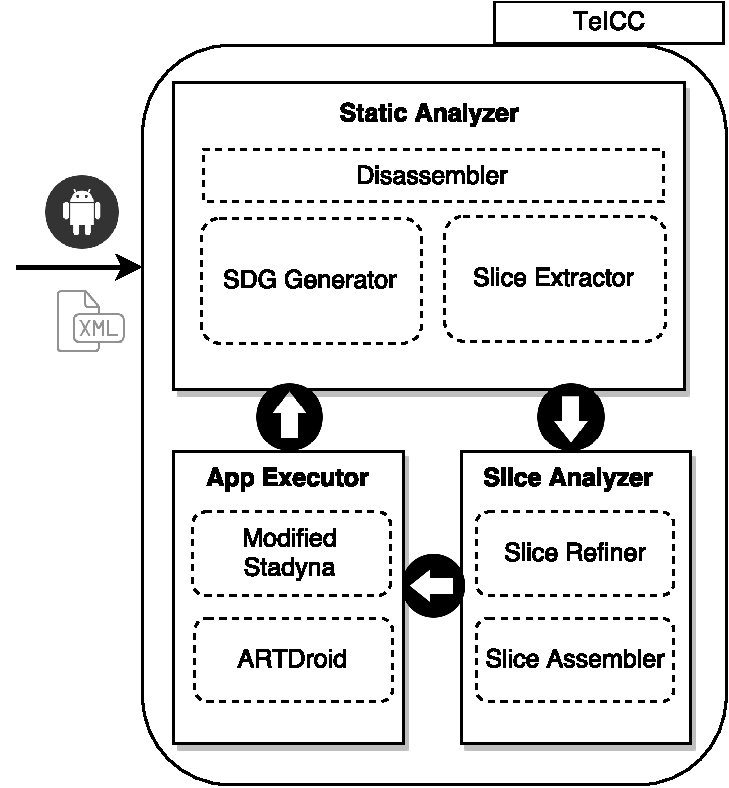
\includegraphics[width=5cm, height=5cm]{T-T}%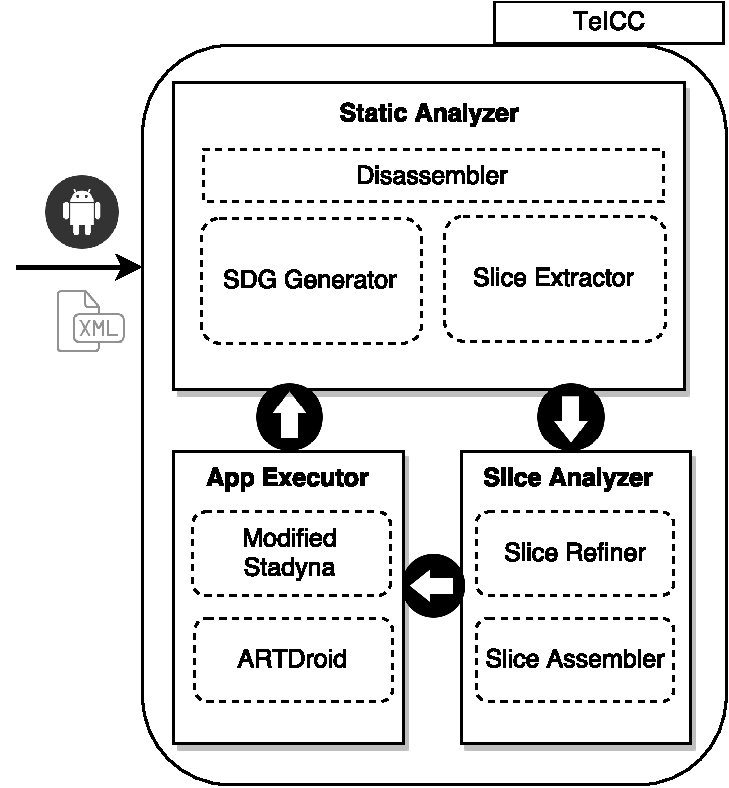
\includegraphics[scale=0.4]{T-T}
\caption{TeICC Design}
\label{fig:design}
\end{figure}



Figure~\ref{fig:design} illustrates a high level design of TeICC. TeICC consists of a Static Analyzer, a Slice Analyzer and an App Executor module. The Static Analyzer further relies on a disassembler to convert an app's compiled Dalvik bytecode to Smali code \cite{Smali}. The Smali files are then taken as input by the SDG Generator to create the first iteration of a SDG. The Slice Extractor assisted by the SDG performs backward program slicing on the Smali files to extract target slices, for the list of MOIs provided as an XML file, across multiple components. The Slice Analyzer module refines the slices by removing irrelevant instructions and merging them in the resultant components as shown in Listing~\ref{lst:slices}. The Slice Assembler part of this module assembles the modified app Smali files and signs the APK file. 



The App Executor module takes the app under analysis as input and installs it on a device for dynamic execution of the target slices. The purpose of the execution of target slices is two-fold. One for de-obfuscation and resolving the targets of dynamic code updates, such as reflection and dynamic class loading. The other purpose is to capture any sensitive/malicious behavior. For handling dynamic code updates, we utilize a modified version of Stadyna~\cite{zhauniarovich2015stadyna} that can resolve the targets of reflection and handle the code loaded dynamically. In order to capture sensitive behavior of app, we leverage an API hooking tool, ARTDroid\cite{costamagnaartdroid}, to hook sensitive APIs such as the \texttt{sendTextMessage()} API. 


\subsection{Enhancement to Backward Slicer}

Our backward slicing mechanism is based on an enhanced version of SAAF which performs static analysis of Android apps on Smali code \cite{hoffmann2013slicing}. We added certain features to it to overcome some of its limitations. 

We extended SAAF to perform backward slicing across multiple components. This extended backward slicing is guided by a SDG when the start of a component is encountered. The backward slicing process continues until it reaches an entry point of the app according to the SDG. The entry point is a node in the SDG which has no predecessor. Moreover, we added a slice extraction feature to SAAF, \textit{i.e.}, to mark all the instructions in the backward slice and write them to another file for further analysis.   

Apart from extending backward slicing to cover ICC, we added other features which are important for the soundness of static analysis. The most important features we added are path-, context- and object-sensitivity \cite{li2016static}. Context- and object-sensitivity is essential to extracting slices across multiple components. We also utilize path-sensitivity where the conditions leading to different paths are resolvable. In cases where these conditions are not resolvable, we use an approach similar to the one used in \cite{rasthofer2016harvesting}.

\subsection{Capturing Dynamic Behavior}

The idea behind a multiphase iterative model is to overcome the shortcomings of both static and dynamic analysis. TeICC relies on a modified version of Stadyna to handle reflection and dynamic code loading\cite{zhauniarovich2015stadyna}. Originally, Stadyna is based on modifications to Android framework (Android 4.2) to resolve the targets of reflection and integrate the code loaded dynamically to the original code base for further static analysis. We  re-implemented Stadyna removing the need of Android framework modification by using ARTDroid. 

We used ARTDroid to hook framework APIs used for dynamic code updates as well as those responsible for sensitive behavior. By intercepting calls to the dynamic code APIs, App Executor provides a feedback to the Static Analyzer for improved creation of SDGs and extended backward slices. In addition, sniffing on sensitive API calls enables TeICC to put a check on suspicious app behavior.       
